%!TEX root = report.tex
\newpage
\section{Echo-SLAM}

\subsection{Sine Sweep Generation}

A common signal for recording room impulse responses is the sine sweep. 
Since for the scale of the present setup, mostly low frequencies are of interest, a signal with exponential increase of frequencies is chosen, ranging from$f_1=100 \text{ Hz}$ to $f_2=20000 \text{ Hz}$, generated by 
\begin{equation}
    x_{exp}(i) = fac \times amp \times \sin(\frac{2 \pi f_1 N}{F_s log(\frac{f_2}{f_1})}  (e^{\frac{i}{N}log(\frac{f_2}{f_1})} - 1)), \quad \text{ for $i = 0 \cdots N$ ,}
    \label{}
\end{equation}

where $N=T_{in} F_s$ is the nubmer of samples and $F_s$ is the sampling frequency. The Fourier transform visualizes the richness of the signal in low frequencies (Figure \ref{fig:sweep_fft}) and the spectrogram provides a more intuitive visualization in time (Figure \ref{fig:sweep_spectrogram}).

The data type of the wavfile is signed integer of 16 bits because it can be read by \texttt{PyAudio}. Hence, the signal is amplified by $amp=2^{16-1}$ and damped with a factor of $fac=0.8$. 

To avoid a too abrupt start which the speakers would not be capable to reproduce, a \textit{Hanning} window is applied to the start of the signal (see Figure \ref{fig:sweep_start}).

\begin{figure}[htb]
	\centering		
	\begin{subfigure}[b]{0.7\linewidth}
        \centering
		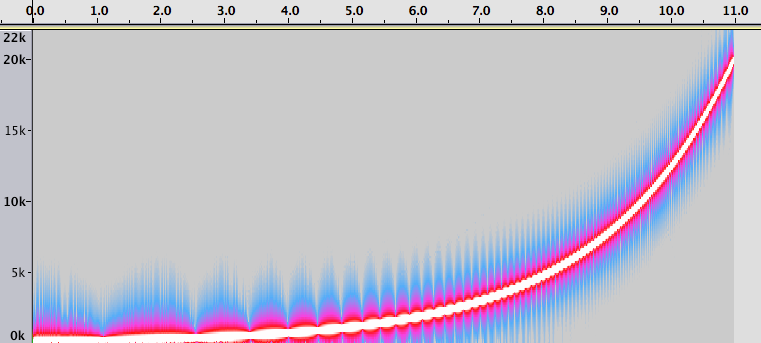
\includegraphics[width=\linewidth]{files/sweep_spectrogram.png}
        \caption{Spectogram of sine sweep.}
        \label{fig:sweep_spectrogram}
	\end{subfigure} \\
	\begin{subfigure}[b]{0.49\linewidth}
        \centering
		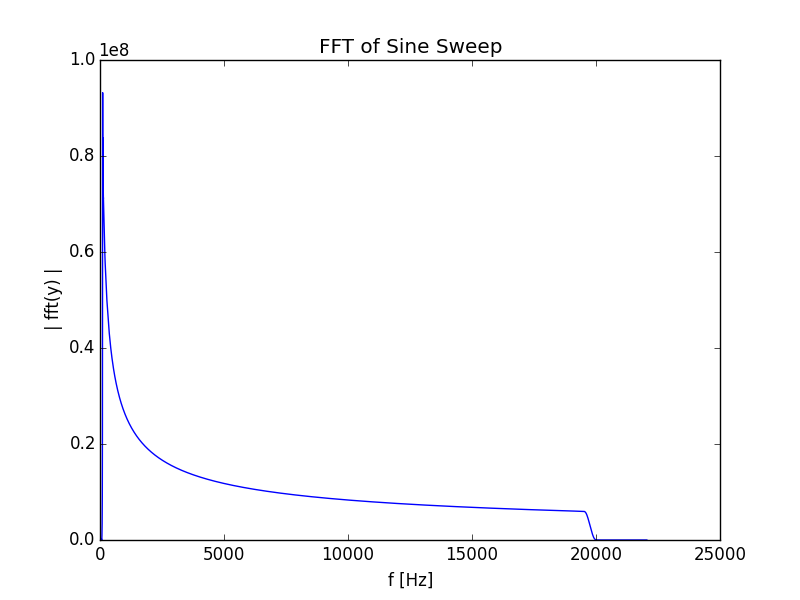
\includegraphics[width=\linewidth]{files/sweep_fft.png}
        \caption{DFT of sine sweep.}
        \label{fig:sweep_fft}
	\end{subfigure}
	\begin{subfigure}[b]{0.49\linewidth}
        \centering
		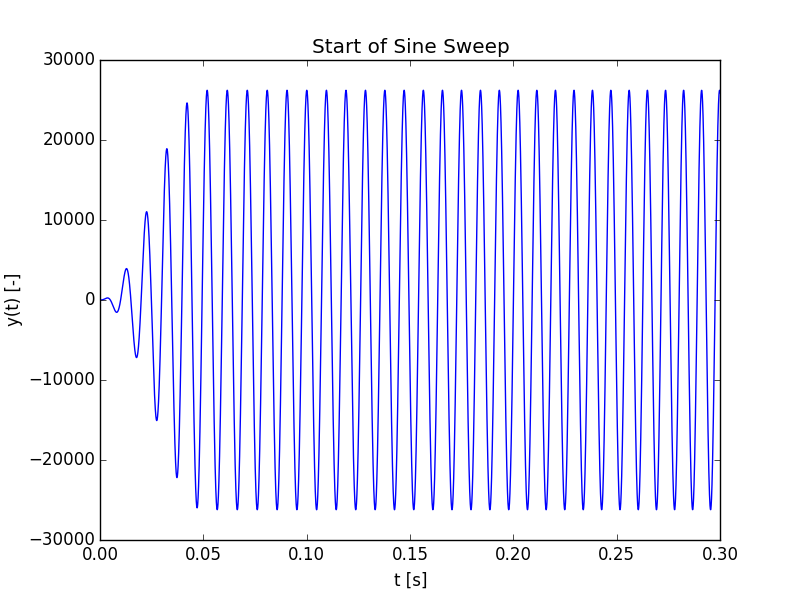
\includegraphics[width=\linewidth]{files/sweep_start.png}
        \caption{Zoom of smoothened start of sine sweep.}
        \label{fig:sweep_start}
	\end{subfigure}
	\caption{Characteristics of sine sweep used for room impulse response recording.} 
	\label{fig:sweep}
\end{figure}

\subsection{Recording}

The recording of the impulse response is implemented in a \texttt{python} script using the library \texttt{PyAudio}. 
All frames are read from the input file and sent to the output stream for a duration of $T_{in}$. 
Simulataneously, the data is read from the input stream for a duration of  $T_{out}=T_{in} + \Delta T$, where $\Delta T$ is fixed at 3 seconds. The incoming data can be read from multiple channels ($N_{channels}$). 
The data is stored in a matrix of size $N_{Buffers} \times (N_{Channels} \times  S_{Chunks})$, where $S_{Chunks}$ denotes the number of bits (1024) and $N_{Buffers}$ denotes the number of buffers, calculated from $N_{Buffers} = T_{out}{F_s}/S_{Chunks}$.
%TODO: test this
The frames from the different channels are stored in alternating order and need to be \"unwrapped\" for storage in separate files. The resulting data matrices are single-channeled and of size $N_{Buffers} \times  S_{Chunks}$.


\subsection{Experimental Results}

\subsubsection{Calibration}
It is required to differentiate the delay induced by the physical distance between microphone, walls and the speakers from the delay induced by the audio system itself. 
Therefore an analysis of the latency of the audio system is performed. 

The speaker is placed at a well known position with respect to the microphone, so that the physical delay $\Delta t_{ph}$ can be precisely calculated. 
It is then sufficient to get the total delay of the signal, $\Delta t_{tot}$ which is composed of the physical delay and the latency ($\Delta t_{tot}=\Delta t_{ph}+\Delta t_{l}$).

The total delay is found by sending a reference signal $u[k]$ (in this case, an approximation of white noise) and recording the response of the microphone, $y[k]$. 
The white noise is generated with a randomn signal of length $T=1\text{ s}$ at a sampling frequency of $F_s=44.1 \text{ kHz}$. Its histogram and Fourier transform are shown in Figures \ref{fig:random_hist} and \ref{fig:random_fft} respectively. 

\begin{figure}[htb]
	\centering		
	\begin{subfigure}[b]{0.49\linewidth}
        \centering
		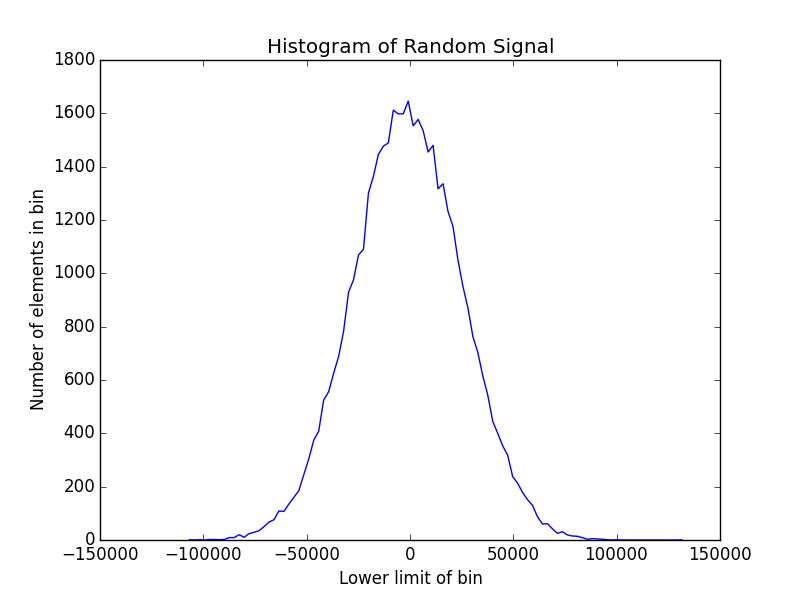
\includegraphics[width=\linewidth]{files/random_hist.png}
        \caption{Histogram}
        \label{fig:random_hist}
	\end{subfigure} 
	\begin{subfigure}[b]{0.49\linewidth}
        \centering
		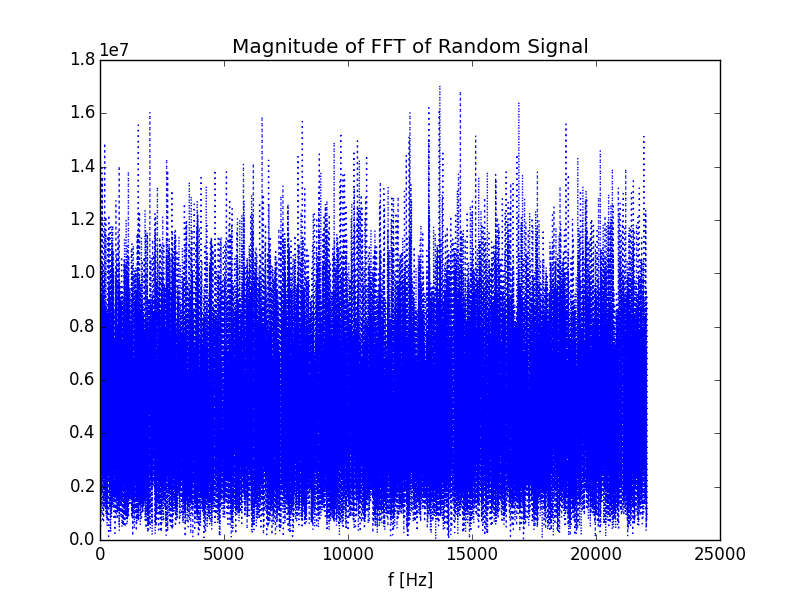
\includegraphics[width=\linewidth]{files/random_fft.png}
        \caption{Magnitude of DFT}
        \label{fig:random_fft}
	\end{subfigure}
    \begin{subfigure}[b]{0.49\linewidth}
        \centering
        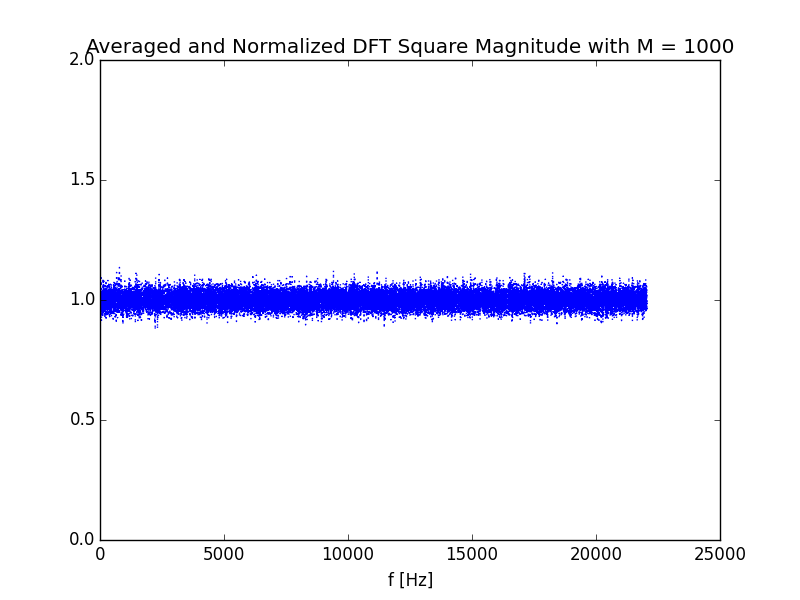
\includegraphics[width=\linewidth]{files/random_M1000.png}
        \caption{Averaged Squared Magnitude of DFT with M=1000}
        \label{fig:random_M1000}
    \end{subfigure}
    \begin{subfigure}[b]{0.49\linewidth}
        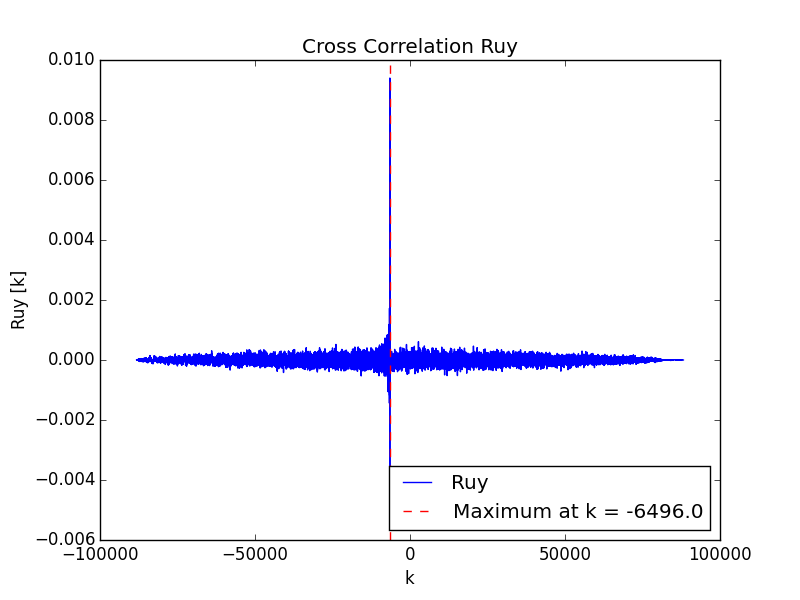
\includegraphics[width=\linewidth]{files/audio_ruy.png}
        \caption{Cross correlation for latency estimation}
        \label{fig:audio_ruy}
    \end{subfigure}
    \caption{Characteristics of random signal used for calibration.} 
	\label{fig:random}
\end{figure}

The power spectral density $P(k)=E(|X_N[k]|^2/N)$ of this signal should be equal to its standard deviation $\sigma^2$ if it is indeed a perfect randomn signal, meaning that its frequency is equally distributed over all frequencies \cite{Vetterli}.
When averaging over 1000 iterations of randomn signal generation, the obtained averaged squared magnitude, normalized by the standard variance, is close to 1 for all frequencies (see Figure \ref{fig:random_M1000}), so the randomness is achieved.

The response is a scaled and delayed noisy version of the input. 
Finding the delay is equivalent to laying the output signal over the input signal with different phase lags until one gets a maximum similarity. The lag corresponding to this maximum is the total delay between the input and the output. The tool that performs these steps is the cross-correlation, which, for discrete signals is 

\begin{equation}
	r_{uy}[k] = \sum\limits_{n=-\infty}^{\infty} u[n]y^*[n-k], \hspace{2em} k=0,\pm1,\pm2,\cdots .
\end{equation}

As the cross-correlation is computationally expensive, only the first $N_{max}$ samples of both input and output signals are correlated, which is sufficient if $N_{max}$ is chosen significantly bigger than the sample index of the expected delay (e.g. $N_{max}=2  \text{ s} \times F_s = 88200$)

From Figure \ref{fig:audio_ruy}, one can see that the maximum occurs at sample $k_{max}=-6496$, which corresponds to a delay of $\Delta t_{tot}=k_{max}/F_s=147.3 \text{ ms}$. 
The distance between microphone and speaker being $d=660mm$, one finds $\Delta t_{ph} = d/c=1.9  \text{ ms}$, so the estimated latency of the sound system is approximately $\Delta t_{l}=145.4 \text{ ms}$.

\subsubsection{Echo SLAM}

The Room Impulse Reponse $h[k]$ can be calculated from the frequency respose of the input $u[k]$ and of the recorded output $y[k]$ by

\begin{equation}
    h[k] = IDFT\{H[n]\} = IDFT\{\frac{Y[n]}{U[n]}\}.
    \label{eq:impulse}
\end{equation}

The analysis of the impulse response is done for one specific position of the robot. For the first considerations, the microphones are assumed to be omnidirectional and placed in the exact center of the robot. 
The estimated times of arrival can then be found from the robot position and stored in a matrix $U$ following the notation proposed in \cite{Miranda}:

\begin{equation}
    U[n,k]=\tau_{n,k}=\frac{\| \tilde{\mathbf{s}}_{n,k}-\mathbf{r}_{n} \|}{C}=\frac{2d_{n,k}}{C}
    \label{eq:TOA}
\end{equation}

where $d_{n,k}$ denotes the distance between wall $k$ and the robot at position $n$, $\tau_{n,k}$ denotes the corresponding time of arrival and $\tilde{\mathbf{s}}_{n,k}$ and $\mathbf{r}_{n}$ denote the position of the virtual source and the robot respectively. 

\begin{figure}[htb]
	\centering		
	\begin{subfigure}[b]{0.49\linewidth}
        \centering
		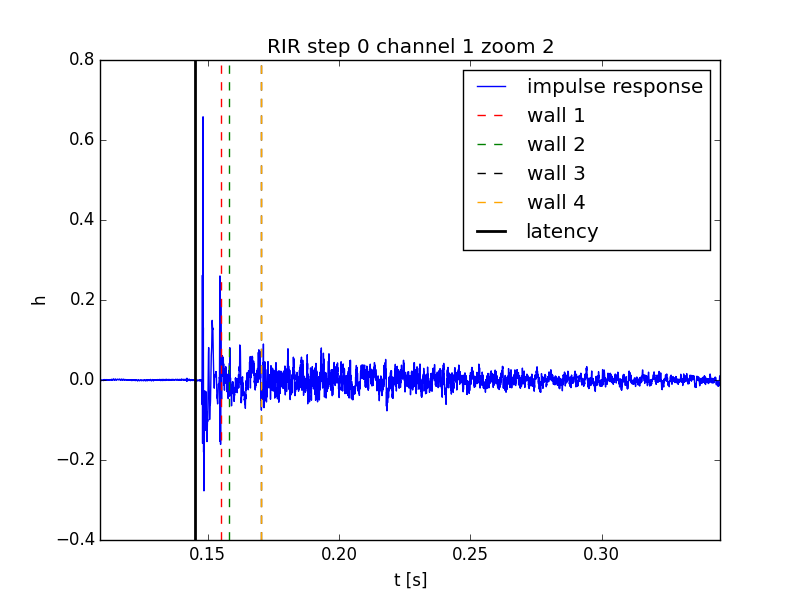
\includegraphics[width=\linewidth]{files/0_1_RIR_zoom2.png}
	\end{subfigure} 
	\begin{subfigure}[b]{0.49\linewidth}
        \centering
		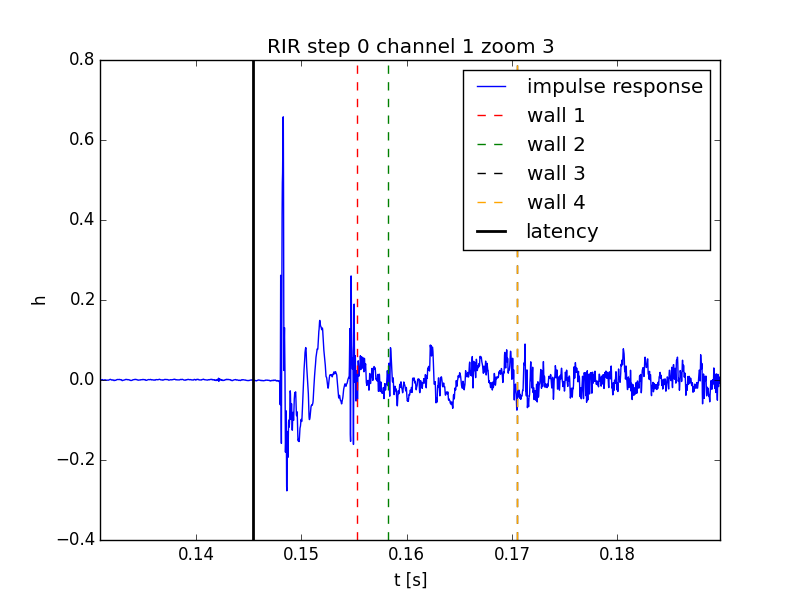
\includegraphics[width=\linewidth]{files/0_1_RIR_zoom3.png}
	\end{subfigure}
	\caption{Room impulse response with estimated times of arrival and latency time.} 
	\label{fig:RIR_zooms}
\end{figure}

These times of arrival are superimposed with the obtained impulse response to find out whether peaks occur where expected (Figure \ref{fig:RIR_zooms}).
One can observe that there are indeed peaks around the expected times, however they are hard to differentiate from other side peaks and noise.

Looking at the frequency spectrum of the recorded response, many peaks at multiples of 108 Hz can be detected (Figure \ref{fig:RIR_filtered}, top plot). 
\begin{figure}[H]
    \centering
    \includegraphics[width=.5\linewidth]{files/notchY.png}
    \caption{Frequency spectrum of recorded response, unfiltered (top) and with applied notch filter(bottom).}
    \label{fig:RIR_filtered}
\end{figure}
These peaks might be the source of unwanted noise and side peaks, which is why an attempt is done to filter them out by applying notch filters on the extraneous frequencies, trying to influence the pertinent frequencies as little as possible. 
A Finite Impulse Response filter (FIR) using a Kaiser Window was first implemented following \cite{notch}, containing few off-frequency ripples and a narrow transient region. 
The filter is applied in forward and backward directions to avoid a phase shift with the filtered data. 
The memory required for the solution of this problem is higher than the memory available in accessible computers. The problem persists when only one forward filter is applied. 

Therefore, a more basic approach is applied, where the unwanted peaks are simply filtered out by setting the response to zero in their neighborhood. The resulting frequency response is shown in Figure \ref{fig:RIR_filtered}, bottom plot). 

Unfortunately, this has no significant effect on the room imuplse response. The reason why the walls are not well detected has not been clearly identified. 
Two possible sources of error could be the following.
Firstly, by construction, the robot obstructs the direct path between walls and the speaker, which could lead to unwanted early echoes and an attenuation of the wall echoes.
Moreover, another error source could be given by non-removable objects in the room. 
It could be observed that different elements of the robot and other loose part such as the speaker itself, the glass wall in the room and other accessories start to vibrate at their own modular frequencies. 
